% Created 2011-05-04 Wed 21:11
\documentclass[11pt]{article}
\usepackage[utf8]{inputenc}
\usepackage[T1]{fontenc}
\usepackage{graphicx}
\usepackage{longtable}
\usepackage{float}
\usepackage{wrapfig}
\usepackage{soul}
\usepackage{amssymb}
\usepackage{hyperref}
\usepackage[spanish]{babel}
\usepackage{bookman}
\usepackage[left=2cm,top=3cm,right=2cm,bottom=1cm,head=1.5cm,includefoot]{geometry}
\usepackage{listings}
\usepackage{multirow}
\usepackage{amssymb}
\usepackage{fancyhdr}
\usepackage{comment}
\usepackage{color}
\usepackage{multicol}
\usepackage[table]{xcolor}
\usepackage{ulem}
\usepackage{pdfpages}

\title{Informe}
\author{}
\date{04 May 2011}

\begin{document}
%Caratula
\thispagestyle{empty}
  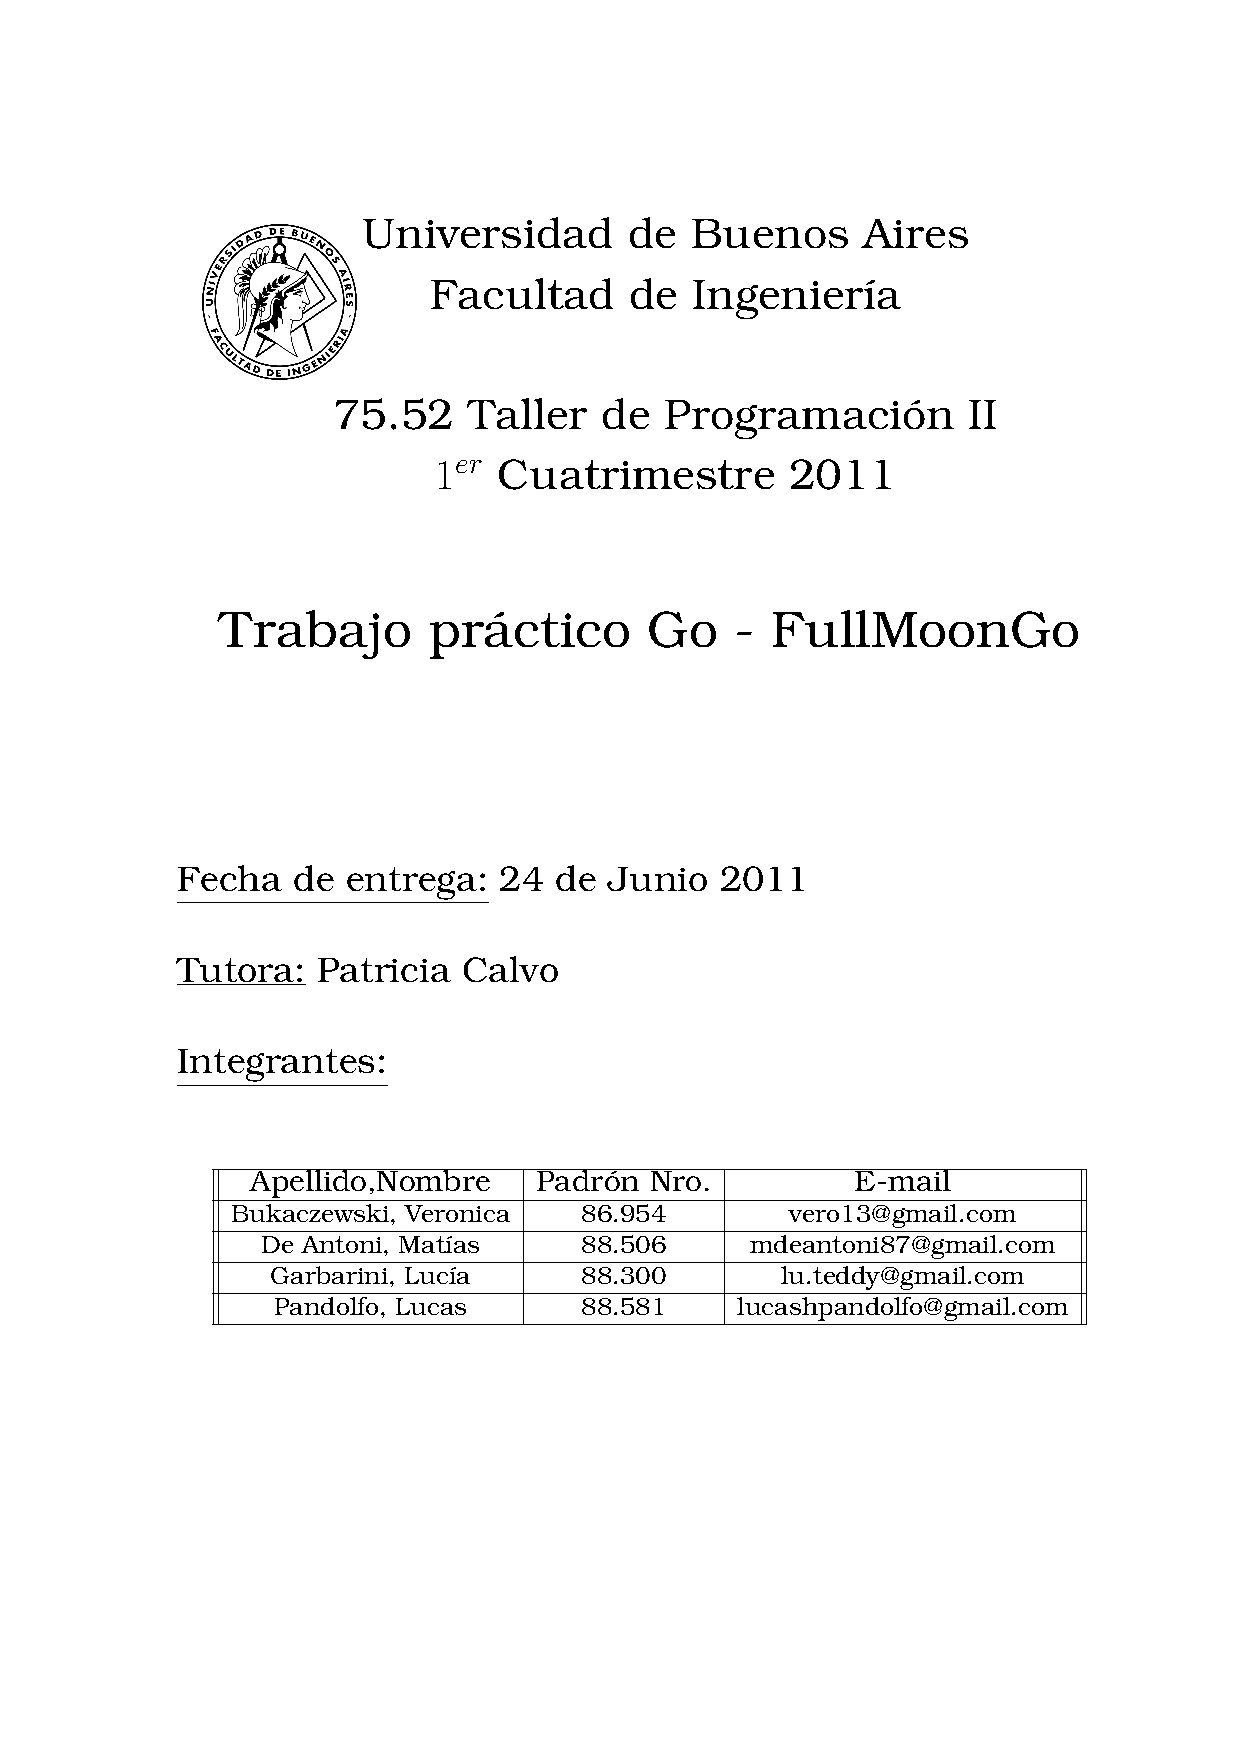
\includepdf[pages=1]{Caratula/Caratula.pdf}

\setcounter{tocdepth}{3}
\tableofcontents
\vspace*{1cm}
\section{Objetivo}
\label{sec-1}

  Desarrollar un sistema que permita jugar partidas de \textbf{Go}, en un
  tablero reducido y considerando el juego finalizado \textbf{a la primera   muerte} (\emph{capture Go}).

\section{Requerimientos funcionales}
\label{sec-2}

  El sistema debe permitir a dos jugadores humanos en la misma
  computadora jugar entre si. También debe permitir como posibles
  participantes del juego a alguna aplicación externa (como ser
  \textbf{gnugo}). Adicionalmente se deben incluír estrategias de juego para
  que una sola persona pueda desarrollar una partida contra el
  sistema.

\section{Manual de usuario}
\label{sec-3}


\section{Detalles de implementación}
\label{sec-4}

\subsection{Vista}
\label{sec-4.1}

\subsection{Protocolo de comunicaciones}
\label{sec-4.2}

\subsection{Estrategias implementadas}
\label{sec-4.3}

   Actualmente se cuenta con cuatro estrategias de juego que serán
   utilizadas posteriormente para elaborar estrategias mas avanzadas:
\subsubsection{EstrategiaComputadoraAtacar}
\label{sec-4.3.1}

    Esta estrategia intenta ocupar casilleros adyacentes a las cadenas
    con menor grado de libertad del oponente, intentando capturarlas.
\subsubsection{EstrategiaComputadoraDefender}
\label{sec-4.3.2}

    Esta estrategia intenta ocupar casilleros adyacentes a las cadenas
    propias con menor grado de libertad, intentando evitar que sean
    capturadas.
\subsubsection{EstrategiaAtaqueCuidadoso}
\label{sec-4.3.3}

    Esta estrategia es una combinación de las estrategias
    ``EstrategiaComputadoraAtacar'' y
    ``EstrategiaComputadoraDefender''. Primero verifica que las
    cadenas propias no estén en peligro de ser capturadas. Si se
    encuentra una cadena propia en riesgo aplica la estrategia
    ``EstrategiaComputadoraDefender'', en caso contrario aplica
    ``EstrategiaComputadoraAtacar''.
\subsubsection{EstrategiaAtaqueCuidadosoMasInteligente}
\label{sec-4.3.4}

    Similar a la estrategia anterior, pero primero verifica si existe
    alguna cadena del oponente con grado de libertad 1. Si existe,
    verifica que ese grado de libertad no se deba a un ojo. Si no se
    deba a un ojo se procede a capturar al grupo. Si no se cumplen
    estas condiciones, se aplica la estrategia
    ``EstrategiaAtaqueCuidadoso''.

\subsubsection{EstrategiaMiniMax}

   Implementa una estrategia del tipo {\bf MiniMax}. En cada turno,
   arma una lista de todos los casilleros vac\'ios y despliega un
   \'arbol de jugadas por cada posible casillero. La profundidad hasta
   la cual despliega el\'arbol de jugadas es configurable. Al llegar a
   la profundidad deseada, se aplica la funci\'on de evaluaci\'on a
   los tableros resultantes.
   
   La funci\'on de evaluaci\'on tiene en cuenta las siguientes
   variables:
   
   \begin{itemize}
      \item Grados de libertad de MAX: Se cuentan todos los casilleros
        adyacentes a cada cadena de MAX libres (no se cuentan los
        repetidos). Se quiere que sea lo mayor posible.
      \item Cantidad de ojos de MAX
      \item Grados de libertad de la cadena mas corta de MAX: la
        variable a la que se le da m\'as importancia.
      \item Grados de libertad de la cadena mas corta de MIN.
      \item Grados de libertad de la cadena mas larga de MIN.
      \item Ojos de MIN.
   \end{itemize}
   
   Por encima de las variables arriba mencionadas, se encuentra la
   condici\'on de que alguna de alguna de las cadenas de MIN tenga
   grado 1. En ese caso se da por ganada la partida (en esa rama del
   \'arbol de jugadas).

   Al desplegar el \'arbol de jugadas, si en alg\'un nivel todos los
   movimientos son inv\'alidos, se da por finalizada la partida y no
   se sigue avanzando hasta los niveles mas profundos.

\subsubsection{Mejoras posibles}

   La implementaci\'on MiniMax presentada se puede mejorar teniendo en
   cuenta lo siguiente:

   \begin{itemize}
     \item Si se es el primero en jugar, no es necesario descender en
       el \'arbol de jugadas. Ser\'ia conveniente comenzar con jugadas
       precalculadas.
     \item Se tienen en cuenta como jugadas posibles todos los
       casilleros libres del tablero. Se podr\'ia tener en cuenta
       solamente los casilleros adyacentes a todas las cadenas
       presentes en el tablero solamente, limitando as\'i las jugadas,
       pero reduciendo el procesamiento, eventualmente d\'andonos la
       posibilidad de descender un poco mas en el \'arbol de jugadas.
     \item La cantidad de niveles que se baja en el \'arbol de jugadas
       es fija. Se puede parametrizar en funci\'on de las jugadas
       posibles. Al principio de la partida, al haber muchas
       posibilidades se elige por ejemplo descender hasta el nivel 3,
       pero a medida que quedan menos posibilidades (la mitad del
       tablero puede ser un caso) podr\'iamos aumentar un nivel sin
       perder mucha velocidad de respuesta.
     \item La funci\'on de evaluaci\'on actualmente es una suma pesada
       de diferentes variables. Se pueden implementar diferentes
       funciones de evaluaci\'on mas sofisticadas.
   \end{itemize}

\end{document}
